%---------------------------------------------------------------------------------------------------------------------!Draft!-----------------------------------------------------------------------------------------------------------------
\subsection{Exemplo de espaço não semi-localmente simplesmente conexo}
\label{não-semi-localmente-simplesmente-conexo-ex}
\begin{titlemize}{Lista de dependências}
	\item \hyperref[espaço-semi-localmente-simplesmente-conexo-def]{Espaço semi-localmente simplesmente conexo};\\ %'dependencia1' é o label onde o conceito Dependência 1 aparece (--à arrumar um padrão para referencias e labels--) 
	%\item \hyperref[]{};\\
% quantas dependências forem necessárias.
\end{titlemize}

\begin{ex}[Brinco Havaiano]
    Brinco Havaiano é a figura construída pela união de círculos $C_n$ que possuem centro $(\frac{1}{n}, 0)$ e raio $\frac{1}{n}$. Isto é, $\underset{n\in \mathbb{N}^*}{\bigcup} C_n$.
\end{ex}


	Toda vizinhança de $0$ contém alguma curva não trivializável.

    De fato, para todo $\varepsilon>0$, $B(0,\varepsilon)$ contém algum círculo de raio menor que $\varepsilon$, pois existe $N\in \mathbb{N}^*$ tal que $\frac{2}{N}<\varepsilon$, isto é, o diâmetro do círculo $C_N$ é menor que o raio de $B(0,\varepsilon)$ e, portanto, $C_N$ está contido em $B(0,\varepsilon)$. 
    
    Uma curva fechada em $C_N$ não é trivializável nem em $B(0,\varepsilon)$ nem em $X$


\begin{figure}[h!]
    \centering
    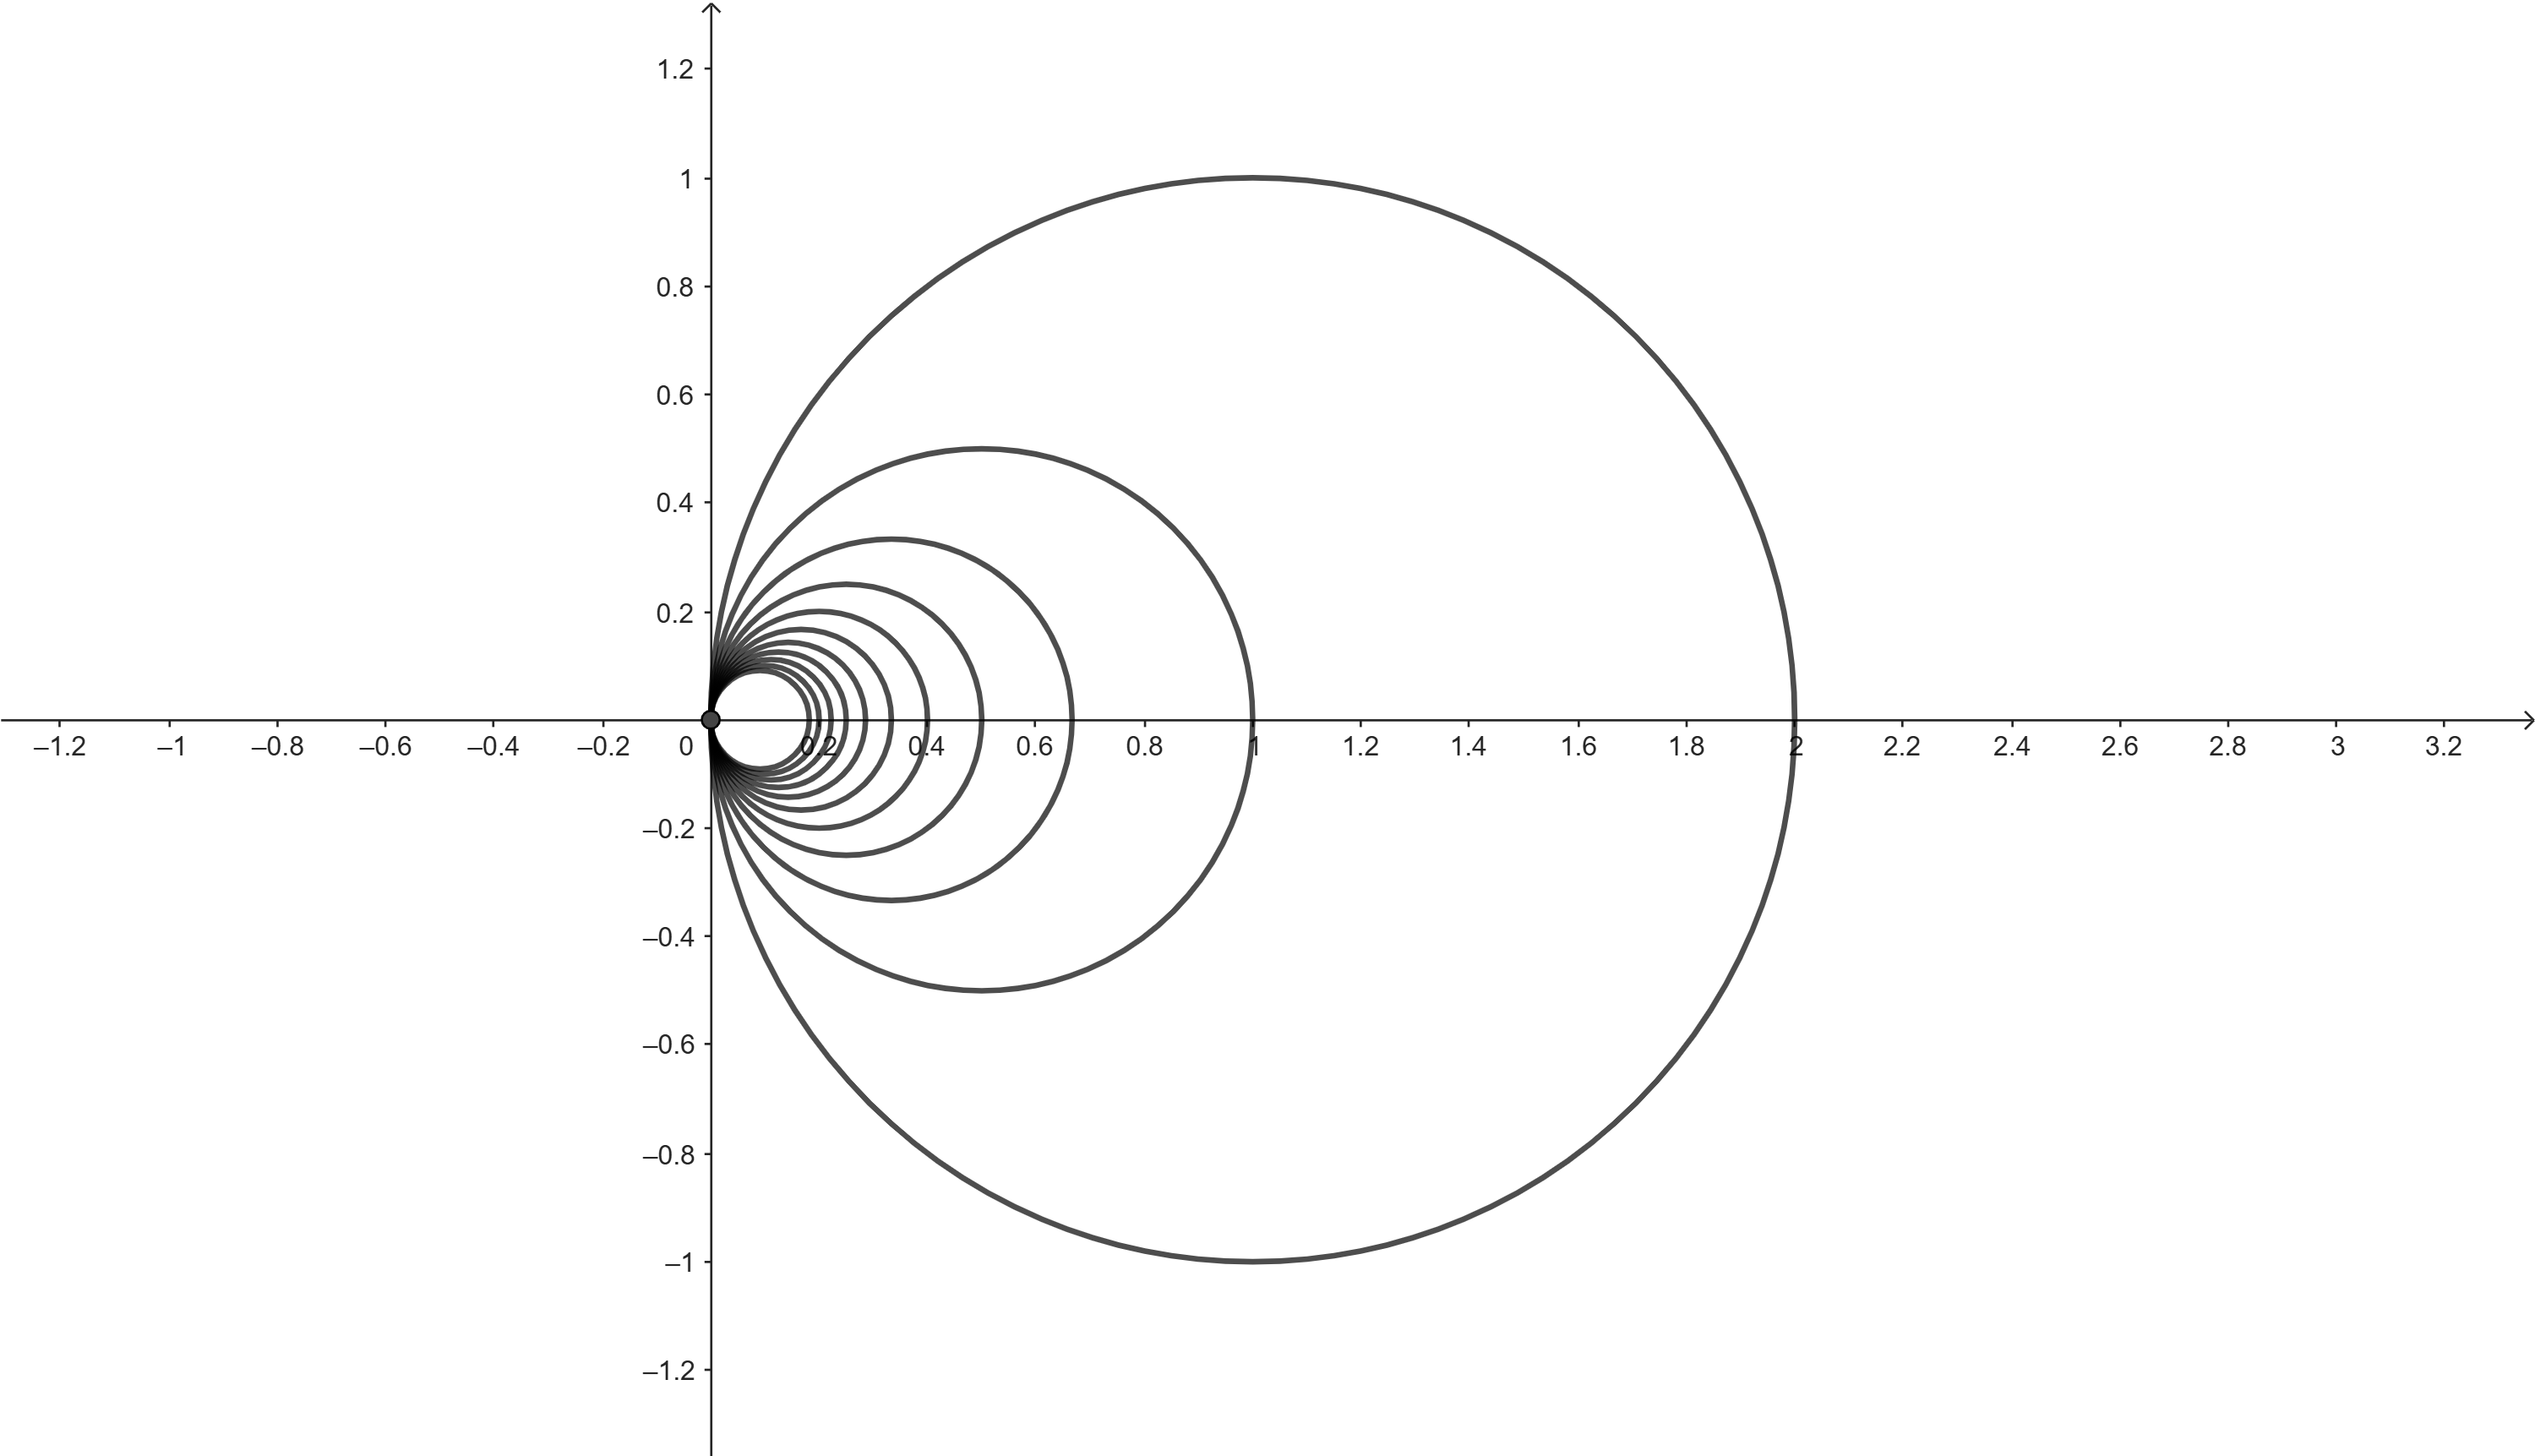
\includegraphics[width=0.8\textwidth]{conteudo/fig-brinco-havaiano.png}
	\caption{Brinco Havaiano}
	\label{fig: brinco havaiano}
\end{figure}





\begin{titlemize}{Lista de consequências}
	\item \hyperref[recobrimento-1-conexo-prop]{Teorema dos recobrimentos 1-conexos};\\ %'consequencia1' é o label onde o conceito Consequência 1 aparece
	%\item \hyperref[]{}
\end{titlemize}
